% Road Accident Severity Prediction with Multimodal Data for Enhanced Road Safety
% BITS Pilani, Dubai Campus -- Foundations of Data Science project report.
% Build:  latexmk -pdf report.tex      (or: pdflatex report.tex, twice)

\documentclass[11pt,a4paper]{article}

\usepackage[T1]{fontenc}
\usepackage[utf8]{inputenc}
\usepackage{lmodern}
\usepackage{microtype}
\usepackage[margin=1in]{geometry}
\usepackage{graphicx}
\usepackage{booktabs}
\usepackage{longtable}
\usepackage{amsmath}
\usepackage{xcolor}
\usepackage{enumitem}
\usepackage{float}
\usepackage[font=small,labelfont=bf]{caption}
\usepackage[most]{tcolorbox}
\usepackage{fancyhdr}
\usepackage{titlesec}
\usepackage[hidelinks,breaklinks]{hyperref}

\definecolor{accent}{HTML}{1F4E79}
\definecolor{rulegrey}{HTML}{BFBFBF}

\titleformat{\section}{\normalfont\Large\bfseries\color{accent}}{\thesection}{0.6em}{}
\titleformat{\subsection}{\normalfont\large\bfseries}{\thesubsection}{0.6em}{}
\titleformat{\subsubsection}{\normalfont\normalsize\bfseries}{\thesubsubsection}{0.6em}{}

\pagestyle{fancy}
\fancyhf{}
\renewcommand{\headrulewidth}{0.4pt}
\fancyhead[L]{\small\itshape Road Accident Severity Prediction}
\fancyhead[R]{\small BITS Pilani, Dubai Campus}
\fancyfoot[C]{\small\thepage}

\setlist[itemize]{topsep=4pt,itemsep=2pt,parsep=0pt,leftmargin=1.4em}
\setlist[enumerate]{topsep=4pt,itemsep=2pt,parsep=0pt,leftmargin=1.6em}

% Framed box used for the pseudocode listings.
\newtcolorbox{algobox}[1]{
  enhanced, breakable, colback=white, colframe=rulegrey,
  boxrule=0.6pt, arc=1pt, left=10pt, right=10pt, top=8pt, bottom=8pt,
  title={\color{accent}\bfseries #1}, coltitle=black,
  colbacktitle=white, titlerule=0pt, fonttitle=\bfseries,
  attach boxed title to top left={xshift=8pt, yshift=-8pt},
  boxed title style={colframe=white, colback=white}
}

\newcommand{\feat}[1]{\texttt{#1}}

\begin{document}

% ------------------------------------------------------------------ title page
\begin{titlepage}
\thispagestyle{empty}
\centering
\vspace*{2.5cm}

{\LARGE\bfseries Road Accident Severity Prediction with\\[0.3em]
Multimodal Data for Enhanced Road Safety\par}

\vspace{2.2cm}
{\large\bfseries SUBMITTED BY\par}
\vspace{0.5em}
\begin{tabular}{l l}
Aarushi Kothari    & 2023A7PS0342U \\
Shreiya Muthuvelan & 2023A7PS0343U \\
Chirudeva Reddy    & 2023A7PS0331U \\
Sanya Wadhawan     & 2023A7PS0296U \\
\end{tabular}

\vspace{1.8cm}
{\large\bfseries SUBMITTED TO\par}
\vspace{0.4em}
{\large Dr.\ Ashish Gupta\par}

\vfill

\includegraphics[width=0.30\linewidth]{figures/bits-logo.png}

\vspace{1.2cm}
{\bfseries BITS PILANI -- DUBAI CAMPUS, DIAC, DUBAI, U.A.E.\par}
\vspace{1cm}
\end{titlepage}

% ------------------------------------------------------------------- contents
\tableofcontents
\newpage

% --------------------------------------------------------------------- part 1
\section{Introduction}

Road traffic accidents remain a major global challenge, inflicting not only severe human loss but
also significant economic losses. With the rapid increase in vehicle density, the frequency and
intensity of traffic collisions have become a major concern. Traditional approaches to traffic
safety remain largely reactive, focusing on post-accident analysis rather than taking proactive
measures.

Through this project we explore the application of machine learning and geospatial analysis to
classify accident severity and identify high-risk, accident-prone areas using the Chicago Crash
Dataset. We intend to develop a tool to equip traffic authorities and policymakers to take
proactive action by integrating explainable AI tools with spatial risk analysis and an interactive
web application.

\subsection{Motivation}

Every year, traffic accidents claim thousands of lives, imposing significant economic burdens due
to injuries and property damage. Two major issues contribute to this challenge:

\begin{itemize}
  \item \textbf{Inability to determine accident severity swiftly.} When an accident is reported,
    emergency teams often rely on incomplete information. Being able to estimate quickly whether an
    accident will result in an injury or not can significantly improve response time and resource
    allocation.
  \item \textbf{Difficulty in identifying accident-prone areas accurately.} Many cities struggle to
    identify which areas consistently experience severe accidents. Without data-driven insights,
    infrastructure upgrades may not be optimally targeted.
\end{itemize}

The motivation behind this project is to address both of these challenges using machine learning
and geospatial analysis.

\subsection{Novelty}

Existing accident analysis systems often lack interpretability and the incorporation of spatial
conditions. The novelty of this project lies in three components:

\begin{itemize}
  \item \textbf{Combining predictive modelling with geospatial analysis.} The model not only
    predicts accident severity but also incorporates spatial clustering, giving insight into which
    localities are prone to accidents.
  \item \textbf{Incorporating interpretability using SHAP and LIME.} Instead of simply outputting a
    prediction about the severity of the crash, the system explains \emph{why} a particular
    prediction was made, highlighting the influence of different features.
  \item \textbf{Development of a web application.} An interactive interface has been developed to
    obtain severity predictions from a set of input conditions.
\end{itemize}

\subsection{Objectives}

This project is designed with the following core objectives:

\begin{itemize}
  \item Build a machine learning pipeline for binary accident severity classification
    (Injury vs.\ No Injury).
  \item Identify key risk factors and explain model predictions through SHAP and LIME analysis.
  \item Perform geospatial analysis to detect crash hotspots and compute risk scores.
  \item Develop an interactive web application for predictions and insights.
\end{itemize}

\newpage
% --------------------------------------------------------------------- part 2
\section{Project Workflow}

\subsection{Block Diagram of the Project}

\begin{figure}[H]
  \centering
  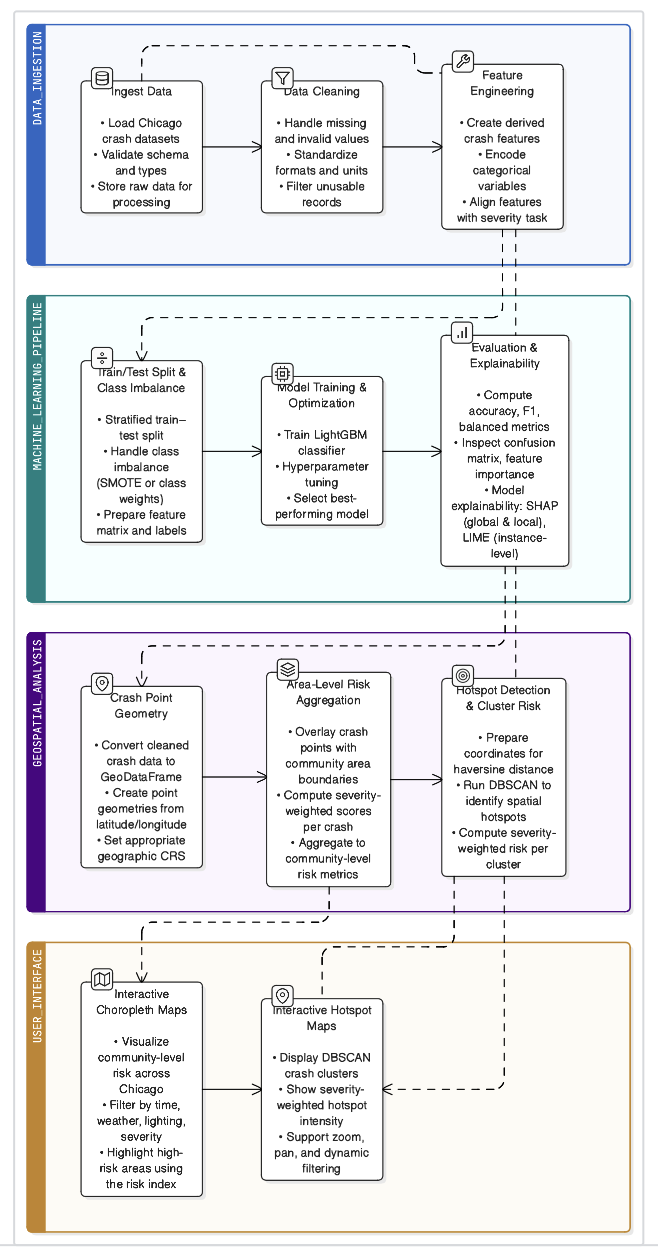
\includegraphics[height=0.82\textheight,keepaspectratio]{figures/workflow.png}
  \caption{End-to-end project workflow: data ingestion, machine learning pipeline, geospatial
  analysis and user interface.}
  \label{fig:workflow}
\end{figure}

\newpage
\subsection{Algorithms Used in the Project}

\subsubsection{Modelling Algorithm}

\begin{algobox}{Algorithm 1 \quad \texttt{modelling.py}}
\textbf{Input:} Raw dataset $D$ with features $X$ and target \feat{CRASH\_TYPE}\\
\textbf{Output:} Trained best model (LightGBM), evaluation metrics, saved artefacts

\medskip
\begin{enumerate}[label=\arabic*.]
  \item Load the libraries required for data processing, modelling, evaluation and saving.
  \item Define project directories for data, models and reports.
  \item $D \leftarrow$ read the CSV file from \texttt{DATA\_PATH}.
  \item Assert that \feat{CRASH\_TYPE} exists in $D$.
  \item $X \leftarrow$ all features without \feat{CRASH\_TYPE}.
  \item $y \leftarrow$ \feat{CRASH\_TYPE}.
  \item Save the label encoder for future inference.
  \item Split $(X, y)$ into $(X_{\text{train}}, X_{\text{test}}, y_{\text{train}},
        y_{\text{test}})$ using a stratified 80/20 train--test split.
  \item Define the preprocessing pipeline:
    \begin{enumerate}[label=(\alph*)]
      \item impute missing numeric values using the \textbf{median};
      \item standardise numeric features.
    \end{enumerate}
  \item Construct a \texttt{ColumnTransformer} applying the preprocessing to all numeric features.
  \item Define the model pipelines:
    \begin{itemize}
      \item $P_1$: Logistic Regression with class weights
      \item $P_2$: Extra Trees Classifier
      \item $P_3$: XGBoost Classifier
      \item $P_4$: LightGBM Classifier
      \item $P_5$: Logistic Regression with SMOTE oversampling
    \end{itemize}
  \item Define the evaluation metrics: \textbf{macro F1 score} and \textbf{balanced accuracy}.
  \item Initialise stratified $k$-fold cross-validation ($k = 5$).
  \item For each model $P_i \in \{P_1, \dots, P_5\}$:
    \begin{itemize}
      \item perform cross-validation on $(X_{\text{train}}, y_{\text{train}})$;
      \item compute the mean macro F1 and balanced accuracy;
      \item store the results in results table $R$.
    \end{itemize}
  \item Identify the best model (\textbf{LightGBM}) from $R$ by highest macro F1 score.
  \item Fit the best model on the full training data $(X_{\text{train}}, y_{\text{train}})$.
  \item Extract the top 20 most important features and save the plot.
  \item Compute the evaluation metrics: test balanced accuracy, test macro F1 and the
        classification report.
  \item Compute the confusion matrix.
  \item Save the best pipeline (\texttt{joblib}), the cross-validation results (CSV) and the test
        metrics (JSON).
  \item Return the final best model, evaluation results and saved outputs.
\end{enumerate}
\end{algobox}

\subsubsection{Geospatial Risk Algorithm}

\begin{algobox}{Algorithm 2 \quad Geospatial risk pipeline}
\begin{enumerate}[label=\arabic*.]
  \item \textbf{Load the pre-processed dataset.}
  \item \textbf{Create the crash GeoDataFrame:} geometry $=$ \texttt{Point(lon, lat)},
        CRS $=$ \texttt{EPSG:4326}.
  \item \textbf{Load the community boundary shapefile:} reproject to \texttt{EPSG:4326} and
        standardise \feat{community\_area\_number}.
  \item \textbf{Spatial join:} join crashes to communities with \texttt{sjoin(POINT within POLYGON)}.
  \item \textbf{Run DBSCAN clustering on the crash coordinates:} obtain the \feat{cluster\_id} for
        each crash and compute the centroid of each cluster.
  \item \textbf{Compute the per-crash severity:}
    \[
      \text{weighted\_severity} =
      \frac{3 f + 2 s + 1 m + 0.5 n}{\text{total\_injuries}}
    \]
    where $f$, $s$, $m$ and $n$ are the fatal, serious, moderate and minor injury counts.
  \item \textbf{Aggregate by community:} \feat{total\_crashes}, injury sums and
        $\operatorname{mean}(\text{weighted\_severity})$; compute the community
        \feat{risk\_index} with the same weighting.
  \item \textbf{Aggregate by cluster:} the same injury sums and \feat{total\_crashes}; compute the
        cluster \feat{weighted\_score} using the risk-index formula.
  \item \textbf{Visualise:} colour-code the map by community risk, and render cluster hotspot maps
        and the interactive Dash dashboard.
\end{enumerate}
\end{algobox}

\newpage
% --------------------------------------------------------------------- part 3
\section{Experimental Results}

\subsection{Cross-Validation Model Performance Comparison}

\begin{table}[H]
  \centering
  \caption{Stratified 5-fold cross-validation results (\texttt{reports/cv\_results.csv}).}
  \label{tab:cv}
  \begin{tabular}{@{}lrrrr@{}}
  \toprule
  \textbf{Model} & \textbf{Macro F1} & \textbf{F1 std} &
  \textbf{Bal.\ accuracy} & \textbf{Bal.\ acc.\ std} \\
  \midrule
  Logistic Regression   & 0.7413 & 0.0018 & 0.7847 & 0.0017 \\
  Extra Trees           & 0.7813 & 0.0011 & 0.7702 & 0.0013 \\
  XGBoost               & 0.8037 & 0.0019 & 0.7959 & 0.0023 \\
  \textbf{LightGBM}     & \bfseries 0.8040 & 0.0018 & \bfseries 0.7966 & 0.0020 \\
  LogReg $+$ SMOTE      & 0.7425 & 0.0020 & 0.7850 & 0.0019 \\
  \bottomrule
  \end{tabular}
\end{table}

\begin{figure}[H]
  \centering
  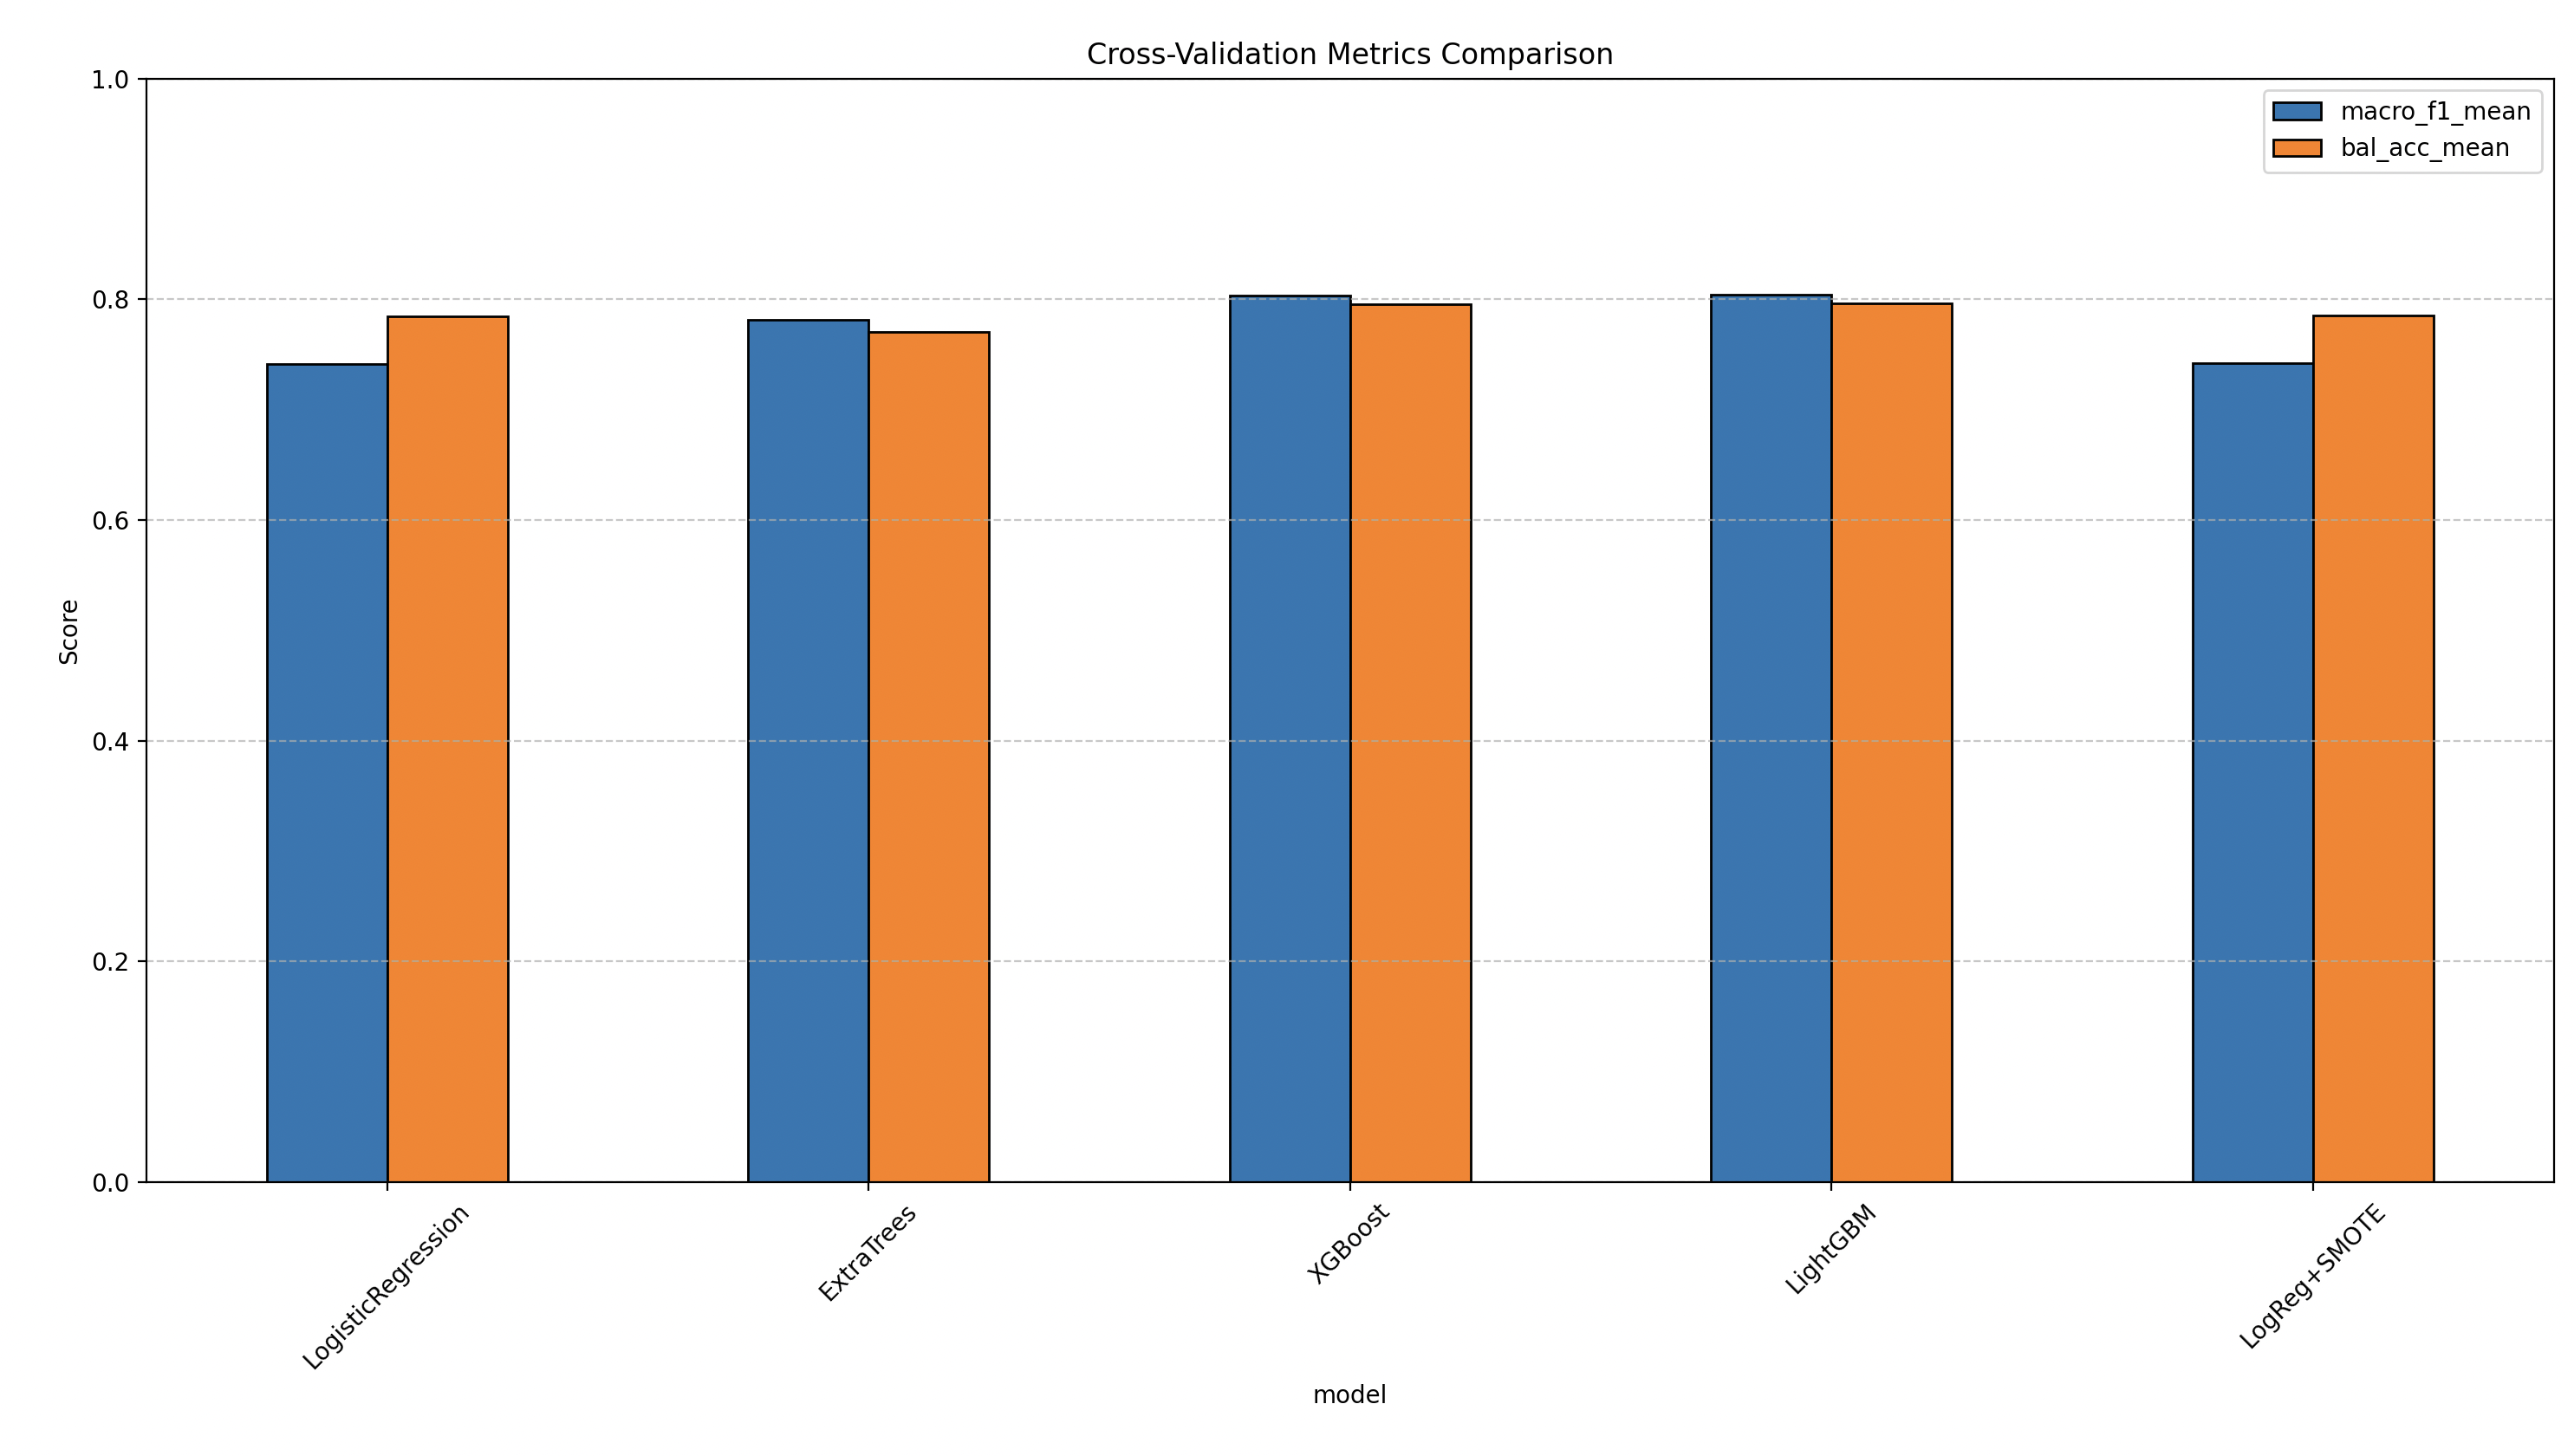
\includegraphics[width=0.92\linewidth]{figures/cv-comparison.png}
  \caption{Cross-validation metric comparison across the five candidate models.}
  \label{fig:cv}
\end{figure}

The cross-validation results compare the macro F1 score and the balanced accuracy of all the
classifiers used in our algorithm, including logistic regression with class weights, Extra Trees,
XGBoost, LightGBM, and logistic regression with SMOTE oversampling. It was observed that the
tree-based ensemble models (Extra Trees, XGBoost and LightGBM) performed better than the linear
models, which suggests that the relationship between the features and accident severity is
non-linear and is captured better by models that model hierarchical feature interactions. The best
chosen model is LightGBM, as it has the highest macro F1 score, making it the most balanced model
for identifying both accident severity classes. Logistic regression with SMOTE shows better
performance than the standard logistic regression model, showing that class imbalance is a factor
affecting performance. Since Extra Trees has built-in class weights, it gives a strong balanced
accuracy score, showing its reliability in handling class imbalance. Overall, the validation
results indicate that the gradient boosting models are the most effective ones for this dataset.

\subsection{Feature Importance Analysis}

The input factors that have the greatest influence on accident severity prediction are highlighted
in the feature importance plot for the best model (LightGBM).

\begin{figure}[H]
  \centering
  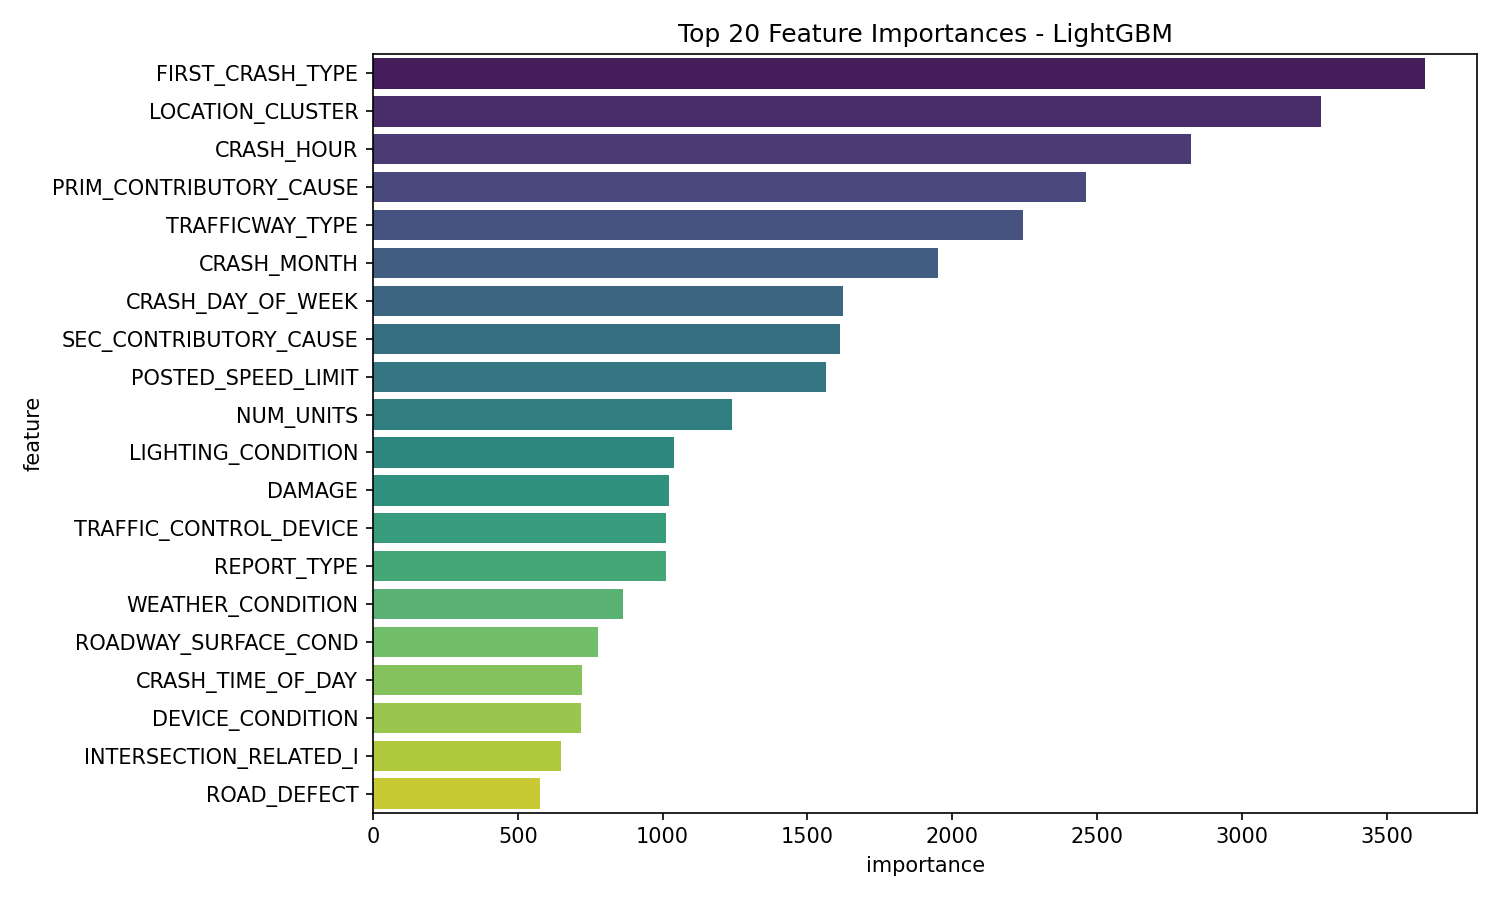
\includegraphics[width=0.92\linewidth]{figures/feature-importance.png}
  \caption{Top 20 feature importances for the LightGBM model.}
  \label{fig:featimp}
\end{figure}

The model relies largely on speed-related and collision-impact factors, showing that accident
dynamics are highly predictive of severity. Features linked to vehicle movement, traffic control
presence and road conditions appear among the top predictors, agreeing with real-world accident
factors. A number of environmental factors, including weather, lighting and road surface, also rate
highly, indicating that external factors affect severe outcomes. Predicting crash severity is
multidimensional, requiring a combination of roadway, environmental and driver-behaviour factors,
as indicated by the presence of multiple mid-importance elements.

\subsection{Confusion Matrix Interpretation}

The confusion matrix below shows how well the model differentiates between the two severity
classes.

\begin{figure}[H]
  \centering
  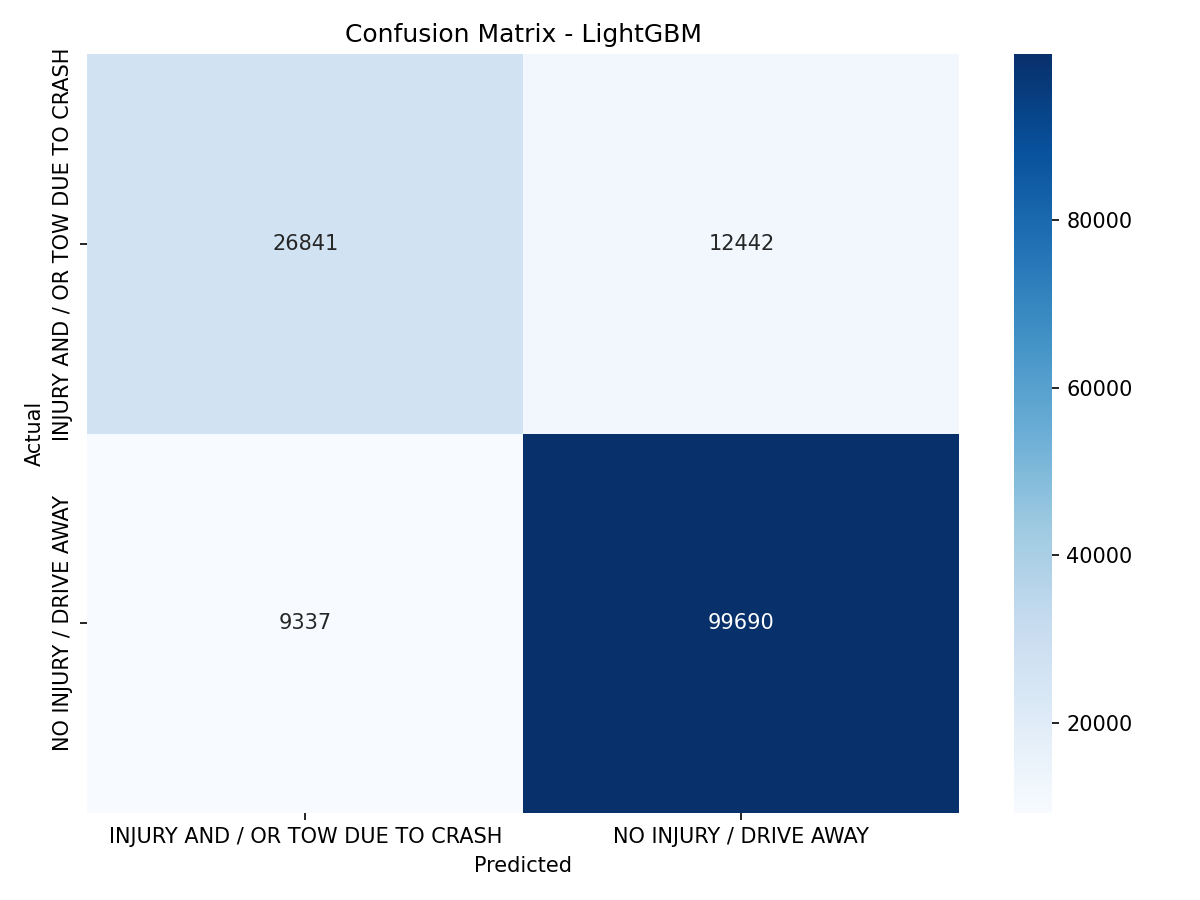
\includegraphics[width=0.78\linewidth]{figures/confusion-matrix.png}
  \caption{Confusion matrix for the LightGBM model on the held-out test set.}
  \label{fig:cm}
\end{figure}

Findings:

\begin{enumerate}
  \item Most samples in both groups are correctly predicted by the model, indicating strong overall
    performance.
  \item The majority of misclassifications happen in the direction of low severity $\rightarrow$
    high severity and vice versa. This is expected, as real-world accident severity commonly lies
    on a continuum.
  \item The comparatively low incidence of false negatives is significant, because under-reporting
    serious accidents could have detrimental effects on public safety.
  \item High diagonal dominance suggests that the classifier generalises well and does not merely
    memorise the training data.
\end{enumerate}

\subsection{Test Performance Metrics}

The final evaluation on the held-out test set
(\texttt{reports/metrics.json}) gives:

\begin{table}[H]
  \centering
  \caption{LightGBM performance on the held-out test set.}
  \label{tab:test}
  \begin{tabular}{@{}l r@{}}
  \toprule
  \textbf{Metric} & \textbf{Value} \\
  \midrule
  Balanced accuracy & 0.7988 \;(79.88\%) \\
  Macro F1 score    & 0.8065 \\
  \bottomrule
  \end{tabular}
\end{table}

Even in the presence of class imbalance, the high balanced accuracy indicates that both severity
classes are reasonably well predicted. The macro F1 score validates that the model maintains
balanced precision and recall rather than favouring the dominant class. The test results are
consistent with the cross-validation findings, demonstrating that the model did not overfit and
generalises effectively.

From the results it is evident that the most dependable and reliable model for predicting accident
severity is LightGBM. Accident severity is controlled by several interacting variables, which makes
tree-based models useful. The model demonstrates strong generalisation ability and performs
consistently across the training, validation and test datasets. Feature relevance aligns with
real-world crash dynamics, adding interpretability to the final model. This establishes the
effectiveness of the selected machine learning approach in predicting accident severity and
highlights the potential for applying the model in traffic safety analytics and roadway risk
assessment.

\subsection{Explainability Methods}

To evaluate whether the LightGBM model was making correct and trustworthy predictions, we
incorporated Explainable AI (XAI) techniques into the analysis. The goal was to understand how the
dataset was being used inside the model and which factors were influencing accident-severity
outcomes. By translating the model's internal mechanics into human-interpretable explanations, XAI
allowed us to assess whether predictions aligned with realistic crash-severity patterns and domain
expectations.

We added explainability because gradient-boosted tree models like LightGBM, while highly accurate,
tend to operate as ``black boxes''. Since our task involves predicting road-accident severity, we
needed to confirm not just strong statistical performance but also that the model's decisions were
grounded in reasonable, interpretable patterns. Hence XAI methods were used to:

\begin{itemize}
  \item check whether the model relied on meaningful accident-related factors (e.g.\ speed, damage,
    number of units);
  \item confirm that predictions were logical for individual samples, especially borderline cases;
  \item translate predictions into actionable insights that could support safety analysis or
    decision-making.
\end{itemize}

To support this analysis, two complementary explainability techniques were applied: SHAP and LIME.
Both methods are widely used in machine learning because they provide structured, interpretable
insights into how models generate predictions. SHAP offers a theoretically grounded framework for
quantifying each feature's contribution, allowing both global patterns and individual decisions to
be examined in a consistent manner. LIME, in contrast, focuses on local interpretability by
approximating the model's behaviour around a specific data point, making it useful for validating
whether individual predictions are based on meaningful and plausible relationships. Together, these
methods help ensure that complex models behave transparently, reveal which inputs drive predictions
and allow practitioners to assess whether the model's reasoning aligns with real-world logic.

\subsubsection{SHAP Analysis}

SHAP (SHapley Additive exPlanations) was used to examine how each feature contributed to the
model's predictions at both the global and local levels.

\paragraph{Globally,} SHAP enabled us to determine which variables consistently exerted the
strongest influence on crash-severity outcomes. Features such as \feat{REPORT\_TYPE},
\feat{NUM\_UNITS}, \feat{DAMAGE} and \feat{POSTED\_SPEED\_LIMIT} showed the highest overall
contributions, confirming that the model relied on meaningful accident-related information rather
than noise or artefacts. A positive SHAP value indicated movement toward the Injury class, while a
negative value pushed the prediction toward No Injury, with the magnitude reflecting the strength of
each effect.

\begin{figure}[H]
  \centering
  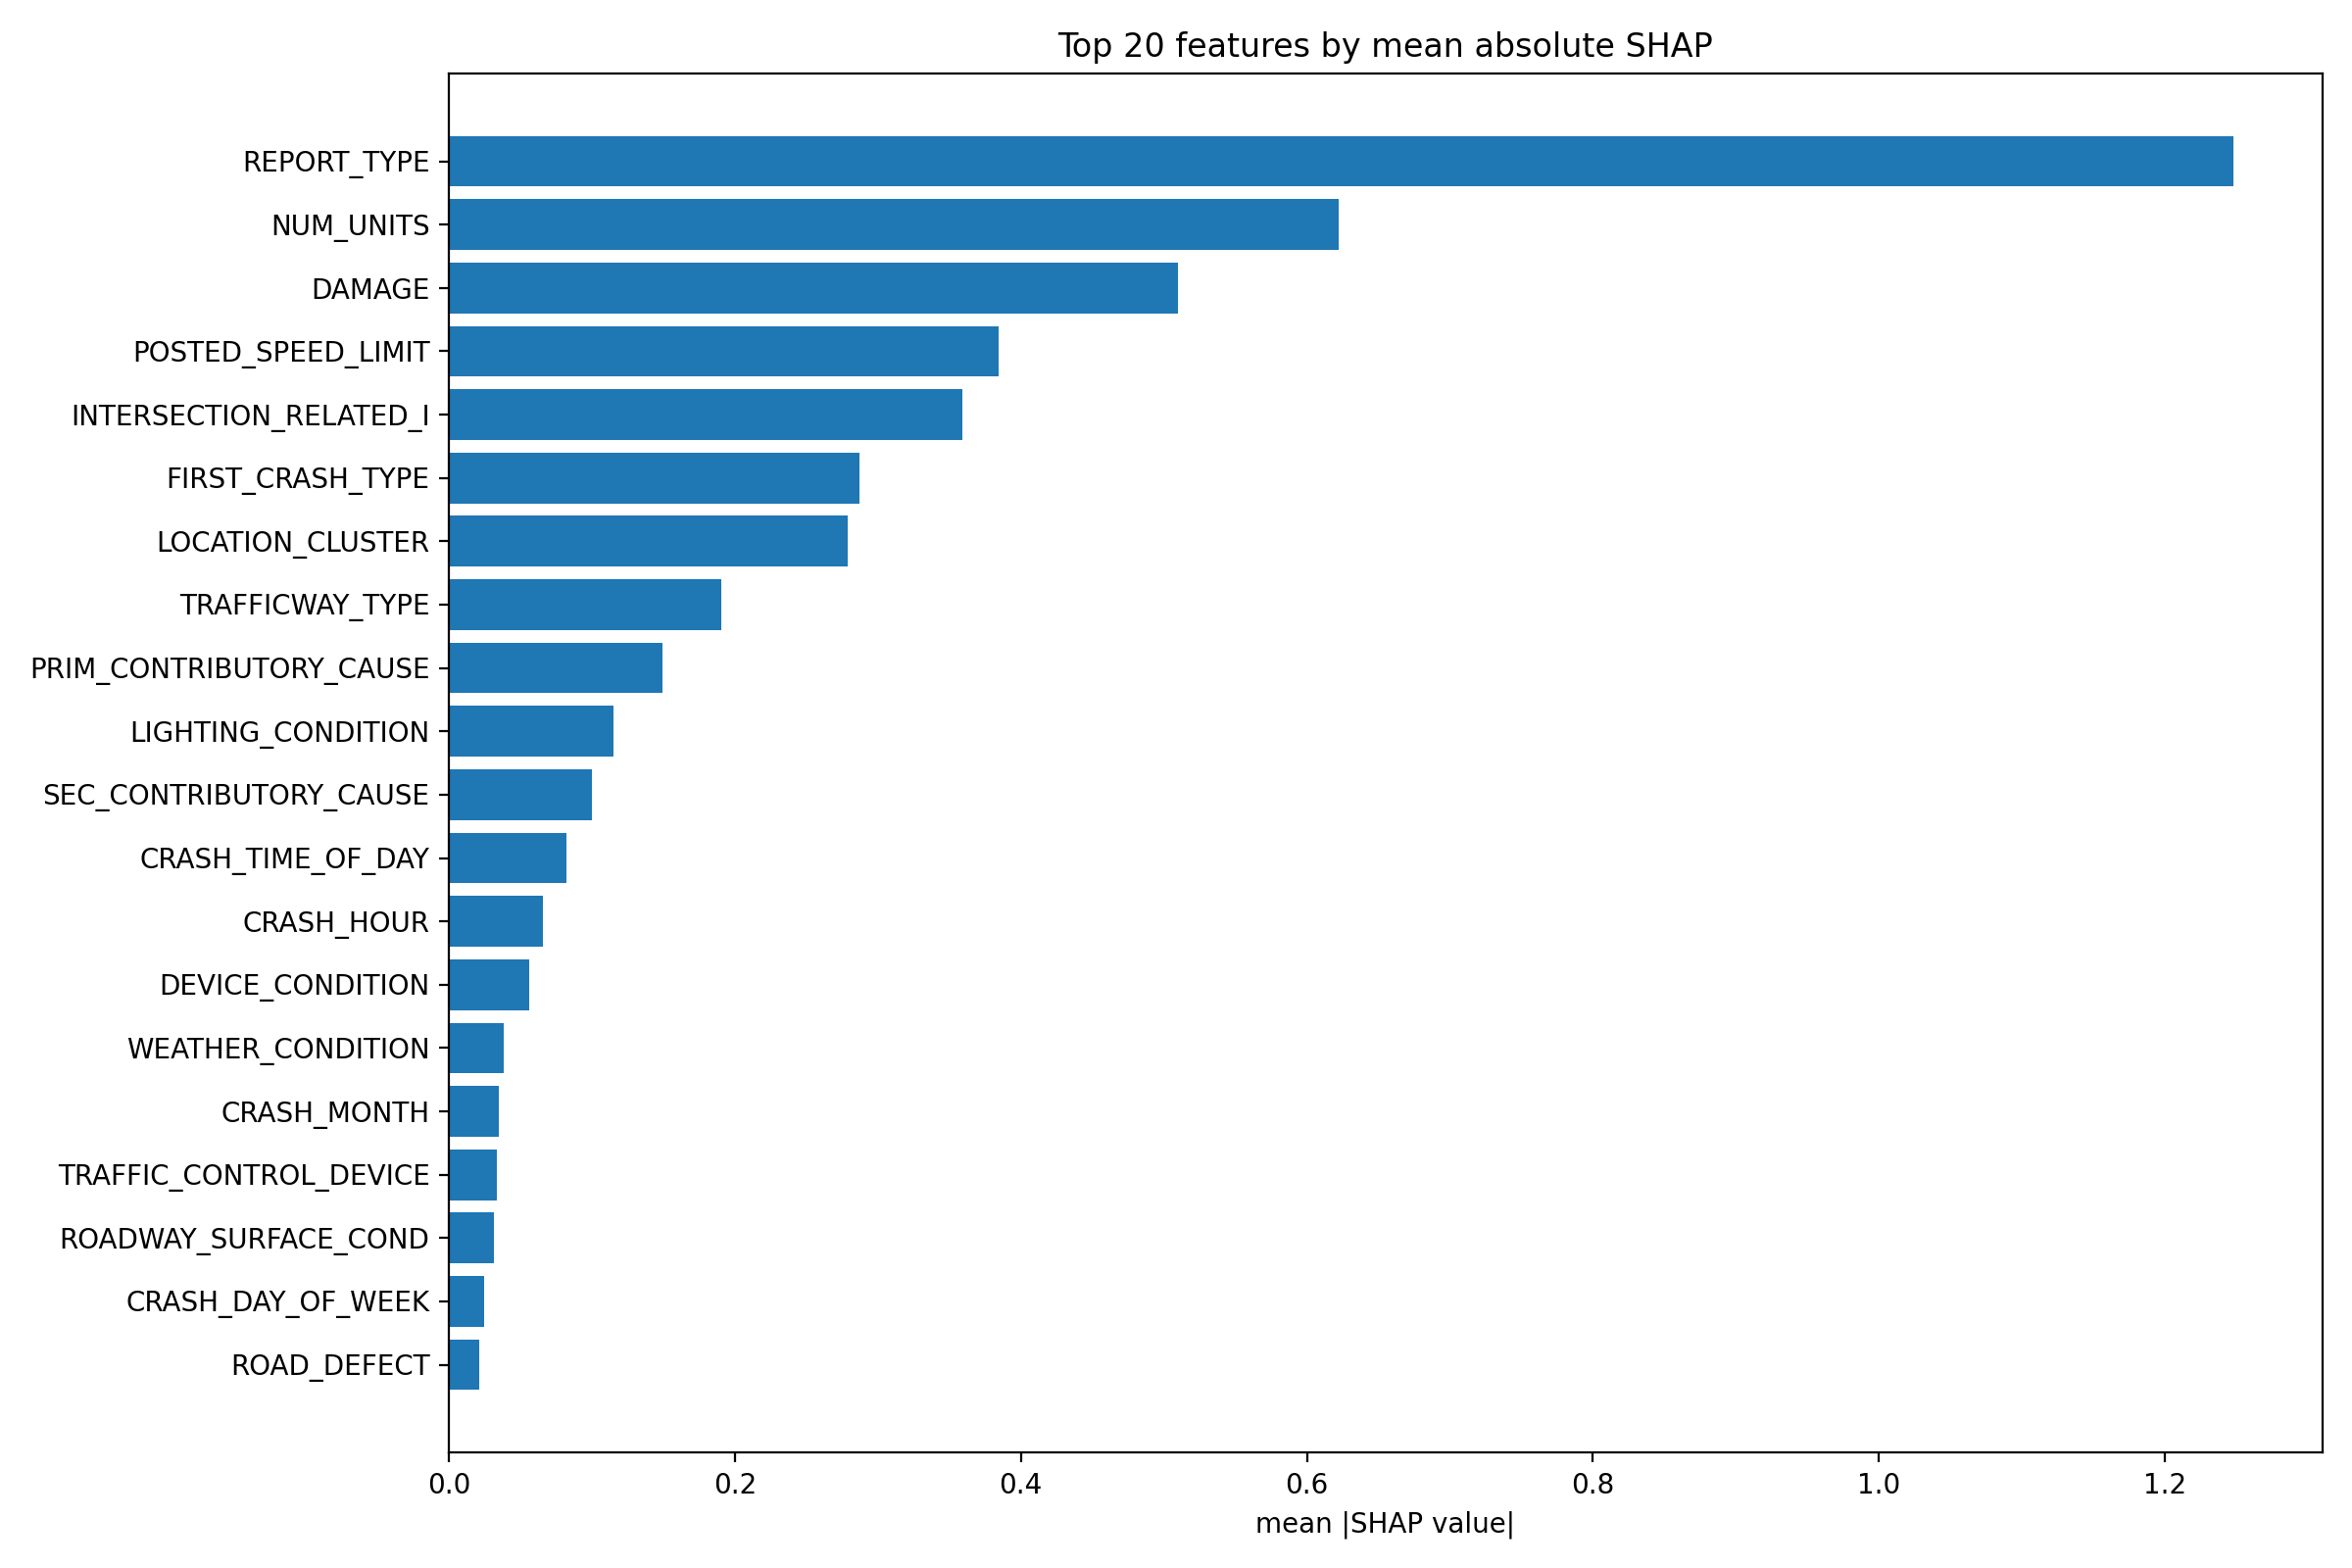
\includegraphics[width=0.92\linewidth]{figures/shap-global.png}
  \caption{Top 20 features by mean absolute SHAP value.}
  \label{fig:shapglobal}
\end{figure}

The results were derived from the average magnitude of SHAP values, and show how strongly each
input variable shaped predictions across the entire dataset. \feat{REPORT\_TYPE} was the most
influential feature, indicating that the type of crash report filed by police was an important
signal for distinguishing between injury and non-injury events, suggesting that incidents formally
documented by police tend to involve more severe outcomes. Features such as \feat{NUM\_UNITS},
\feat{DAMAGE} and \feat{POSTED\_SPEED\_LIMIT} followed closely, reflecting real-world crash severity
outcomes: higher posted speed limits and greater damage levels naturally align with increased
injury likelihood, while simple two-unit collisions tend to reduce predicted severity. The fact
that the strongest SHAP values were concentrated within this small group of features indicates that
the model was focusing on relationships that matter for predicting crash severity, rather than
picking up random patterns in the data. Just as importantly, the very low SHAP values for less
relevant variables showed that those features had little influence on the predictions.

Furthermore, to see clearly how much each feature contributed to the crash, a percent contribution
was calculated for each feature. This was calculated by dividing the mean absolute SHAP value of
that feature by the sum of all mean absolute SHAP values across the sampled predictions. This
approach converts raw SHAP magnitudes into an interpretable metric that expresses how much of the
model's total decision-making ``weight'' can be attributed to each variable. For example,
\feat{REPORT\_TYPE} has a mean absolute SHAP value of 1.25 out of a combined total of 4.63, which
corresponds to approximately 26.93\% of the total influence. Presenting the results in percentages
makes it easier to compare relative importance and identify which features consistently contributed
the most to the model's understanding of injury likelihood. This metric complements traditional
feature importance from LightGBM by grounding the interpretation in the actual direction and
magnitude of contribution toward the severity prediction.

\newpage
\begin{center}
\small
% Generated from road-accident-severity/reports/explainability_outputs/shap_top20_percent.csv -- do not edit by hand.
\begin{longtable}{@{}p{0.30\linewidth}r p{0.52\linewidth}@{}}
\caption{Top 20 features by percent contribution to the model's total SHAP magnitude, with suggested preventive measures.}\\
\toprule
\textbf{Feature} & \textbf{Percent} & \textbf{Suggested preventive measure} \\
\midrule
\endfirsthead
\toprule
\textbf{Feature} & \textbf{Percent} & \textbf{Suggested preventive measure} \\
\midrule
\endhead
\bottomrule
\endfoot
\texttt{REPORT\_TYPE} & 26.93\% & Investigate and apply targeted engineering, enforcement or education depending on feature context. \\
\texttt{NUM\_UNITS} & 13.42\% & Improve intersection control and sightlines; redesign merges/diverges. \\
\texttt{DAMAGE} & 11.01\% & Investigate and apply targeted engineering, enforcement or education depending on feature context. \\
\texttt{POSTED\_SPEED\_LIMIT} & 8.30\% & Lower speed limits where needed; speed cameras and traffic calming. \\
\texttt{INTERSECTION\_RELATED\_I} & 7.76\% & Investigate and apply targeted engineering, enforcement or education depending on feature context. \\
\texttt{FIRST\_CRASH\_TYPE} & 6.19\% & Target high-risk collision types with engineering (roundabouts, protected turns), education and enforcement. \\
\texttt{LOCATION\_CLUSTER} & 6.02\% & Install engineering countermeasures (speed cushions, signage), hotspot redesigns and increased enforcement. \\
\texttt{TRAFFICWAY\_TYPE} & 4.11\% & Road design changes: medians, separated lanes and speed management. \\
\texttt{PRIM\_CONTRIBUTORY\_CAUSE} & 3.23\% & Behavioural interventions: distracted-driving campaigns, DUI checkpoints, enforcement for speeding. \\
\texttt{LIGHTING\_CONDITION} & 2.49\% & Upgrade street lighting and reflective signage. \\
\texttt{SEC\_CONTRIBUTORY\_CAUSE} & 2.16\% & Investigate and apply targeted engineering, enforcement or education depending on feature context. \\
\texttt{CRASH\_TIME\_OF\_DAY} & 1.78\% & Investigate and apply targeted engineering, enforcement or education depending on feature context. \\
\texttt{CRASH\_HOUR} & 1.42\% & Focus lighting, policing and awareness campaigns at high-risk hours. \\
\texttt{DEVICE\_CONDITION} & 1.21\% & Maintain traffic control devices and signals. \\
\texttt{WEATHER\_CONDITION} & 0.83\% & Weather-responsive signage and maintenance in seasonal risk months. \\
\texttt{CRASH\_MONTH} & 0.75\% & Investigate and apply targeted engineering, enforcement or education depending on feature context. \\
\texttt{TRAFFIC\_CONTROL\_DEVICE} & 0.72\% & Investigate and apply targeted engineering, enforcement or education depending on feature context. \\
\texttt{ROADWAY\_SURFACE\_COND} & 0.68\% & Improve pavement maintenance and anti-skid surfacing. \\
\texttt{CRASH\_DAY\_OF\_WEEK} & 0.54\% & Investigate and apply targeted engineering, enforcement or education depending on feature context. \\
\texttt{ROAD\_DEFECT} & 0.46\% & Promptly repair defects and inspect high-risk sections frequently. \\
\end{longtable}

\end{center}

\paragraph{Local interpretability using SHAP.}
SHAP was also used to analyse specific crash samples to understand the exact feature interactions
that led to individual prediction outcomes. Local SHAP explanations provide a \emph{force-plot
representation} where features pushing the prediction toward the Injury class appear in red, and
those pushing it toward the No Injury class appear in blue. The base value represents the model's
expected prediction across the entire dataset, and the final output value results from adding or
subtracting the feature contributions for the selected sample.

\begin{figure}[H]
  \centering
  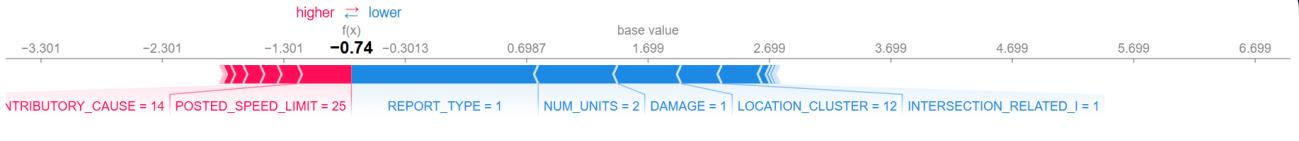
\includegraphics[width=\linewidth]{figures/shap-force.png}
  \caption{SHAP force plot for the test sample at index 10.}
  \label{fig:shapforce}
\end{figure}

For the sample positioned at index 10 in the test set, SHAP revealed that the model predicted a low
likelihood of injury because several strong negative (blue) factors dominated the decision. These
included a low \feat{POSTED\_SPEED\_LIMIT}, a minimal \feat{DAMAGE} level, a benign crash
\feat{REPORT\_TYPE} and a simple two-unit involvement, all of which historically correlate with
non-injury outcomes. Although a few contextual variables such as lighting conditions or trafficway
type pushed the prediction slightly toward the Injury side, their influence was comparatively weak
and insufficient to override the strong indicators of a mild crash. This level of granularity helped
validate that the model's prediction for this specific incident was grounded in a realistic and
contextually coherent explanation.

\subsubsection{LIME Analysis}

LIME (Local Interpretable Model-agnostic Explanations) was used as a complementary technique to
validate the model's reasoning at the individual-case level. Unlike SHAP, which explains model
behaviour across the dataset, LIME constructs a simplified local approximation of the model around
a specific prediction. This allowed us to check whether small, realistic changes in feature values
would meaningfully alter the predicted severity, and whether those changes aligned with
expectations.

\begin{figure}[H]
  \centering
  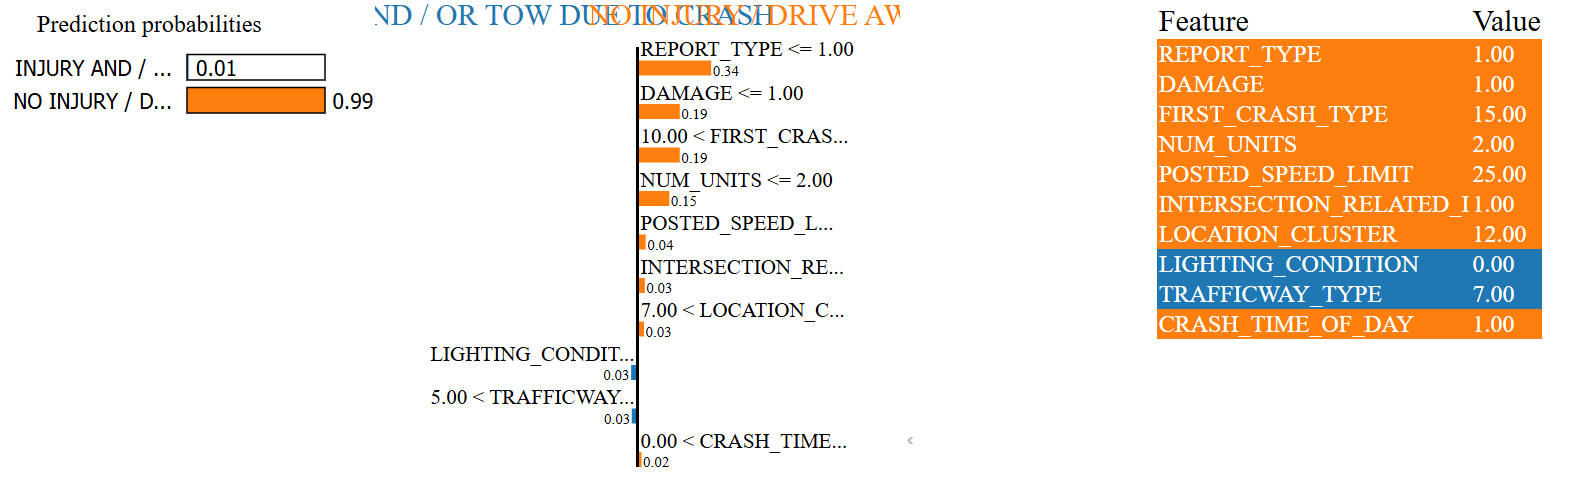
\includegraphics[width=\linewidth]{figures/lime.png}
  \caption{LIME explanation for the same test sample at index 10.}
  \label{fig:lime}
\end{figure}

LIME highlighted a low-severity prediction, meaning the No Injury class. Consistent with the SHAP
results, LIME identified a low \feat{POSTED\_SPEED\_LIMIT}, minimal \feat{DAMAGE}, a typical crash
location and a non-critical \feat{REPORT\_TYPE} as strong indicators of a mild crash. While certain
conditions such as \feat{LIGHTING\_CONDITION} and \feat{TRAFFICWAY\_TYPE} were shown to moderately
increase the predicted severity, LIME's explanation made clear that these factors were outweighed
by multiple dominant features signalling a low-risk event. The convergence between LIME and SHAP
provided strong evidence that the model's prediction for this sample was stable, interpretable and
aligned with domain knowledge.

\subsubsection{Relevance of Explainability to the Overall Analysis}

Using both SHAP and LIME generated a comprehensive, multi-level understanding of why the LightGBM
model behaved the way it did. Globally, the explainability methods demonstrated that the model
relied heavily on logically meaningful features, such as report type, speed limits, number of units
involved and damage severity, when predicting crash outcomes. This confirms that the model was not
driven by noise, spurious correlations or dataset artefacts.

At the local level, SHAP and LIME validated the correctness of predictions for specific crash cases
by exposing the precise variable interactions responsible for the outcome. When both methods agreed
on the reasoning behind a prediction, it strengthened confidence that the model's internal logic was
consistent and trustworthy. This approach was essential for ensuring that the model could not only
achieve strong predictive accuracy but also provide insights suitable for informed decision-making
in road-safety analysis.

Explainability hence helped show that the LightGBM model was a transparent analytical tool capable
of supporting evidence-based discussions about accident severity. The alignment between real-world
crash patterns and the model's inferred logic shows the reliability of its predictions.

\subsection{Geospatial Analysis}

\begin{figure}[H]
  \centering
  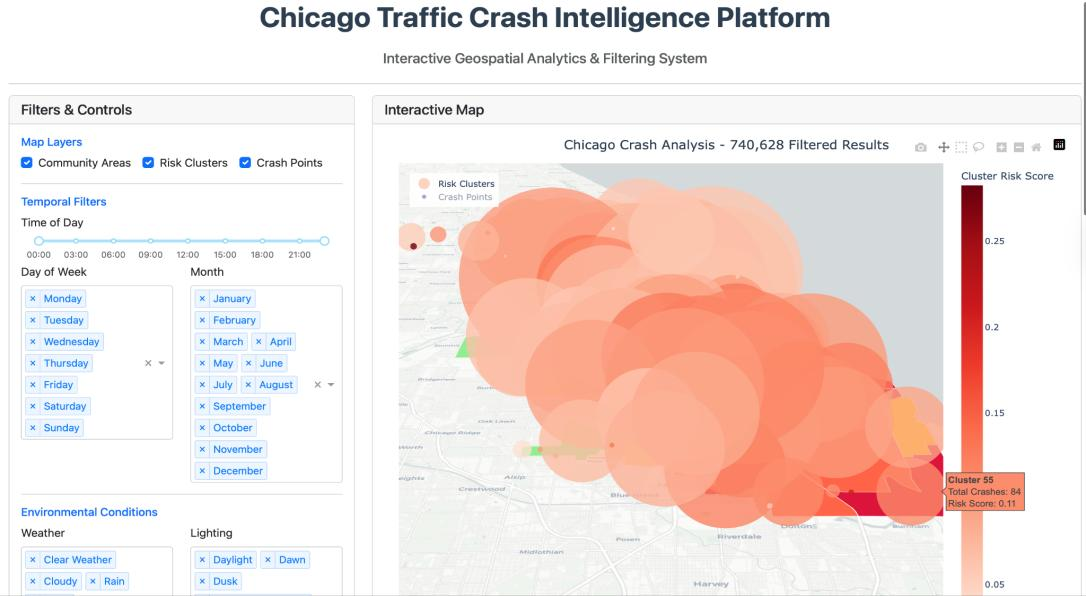
\includegraphics[width=\linewidth]{figures/geo-dashboard.png}
  \caption{Representation of individual clusters and their corresponding risk score.}
  \label{fig:geo1}
\end{figure}

\begin{figure}[H]
  \centering
  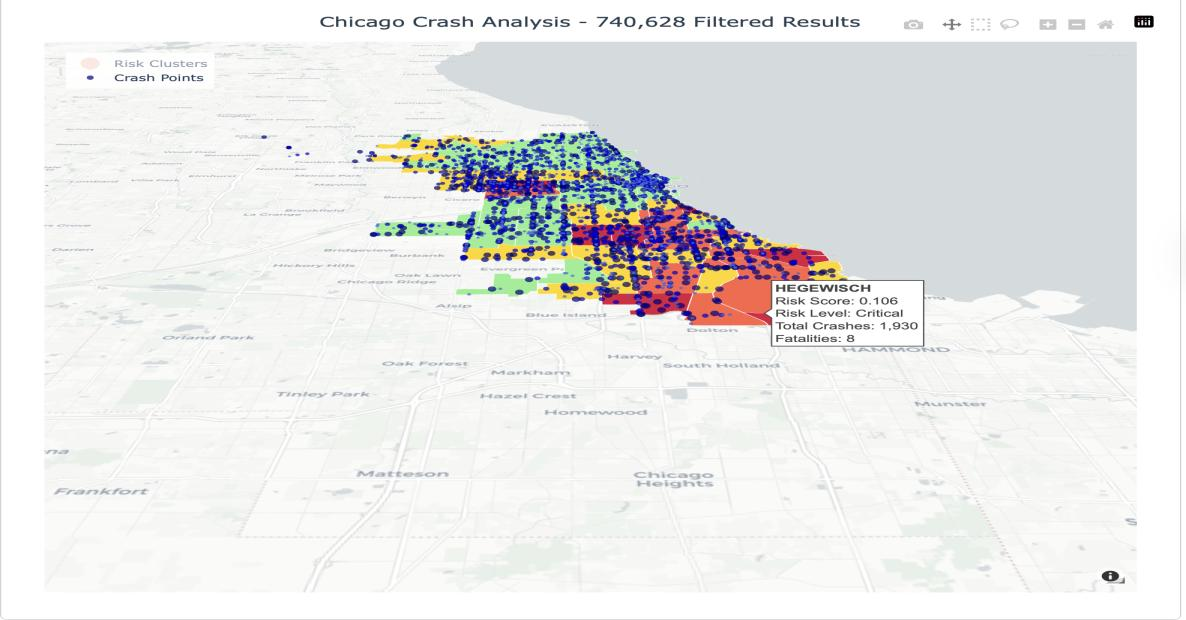
\includegraphics[width=0.95\linewidth]{figures/geo-crashpoints.png}
  \caption{Individual crash points spread out across Chicago.}
  \label{fig:geo2}
\end{figure}

\begin{figure}[H]
  \centering
  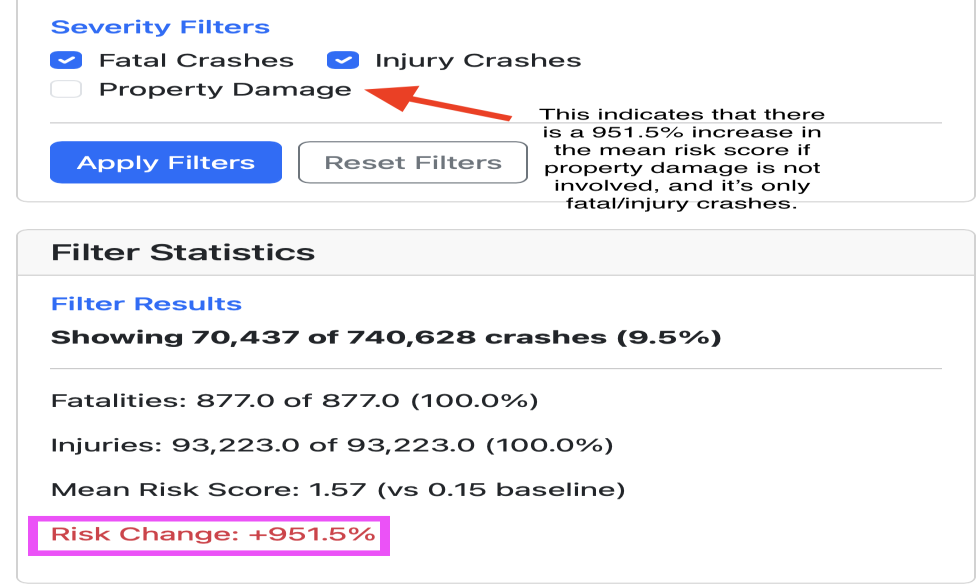
\includegraphics[width=0.82\linewidth]{figures/geo-filters.png}
  \caption{Dynamic modification of parameters leading to a change in the mean risk score. Restricting
  the view to fatal and injury crashes raises the mean risk score from the 0.15 baseline to 1.57,
  an increase of 951.5\%.}
  \label{fig:geo3}
\end{figure}

\end{document}
